\documentclass[problem]{mcs}

\begin{pcomments}
  \pcomment{MQ_matching}
  \pcomment{edited by ARM 10/19/13}
\end{pcomments}

\pkeywords{
  bipartite
  matching
  bottleneck
}

%%%%%%%%%%%%%%%%%%%%%%%%%%%%%%%%%%%%%%%%%%%%%%%%%%%%%%%%%%%%%%%%%%%%%
% Problem starts here
%%%%%%%%%%%%%%%%%%%%%%%%%%%%%%%%%%%%%%%%%%%%%%%%%%%%%%%%%%%%%%%%%%%%%

\begin{problem}

\begin{problemparts}

\problempart Show that there is no matching for the bipartite graph $G$ in
Figure~\ref{fig:bipartite_with_bneck} that covers $\leftbi{G}$.

\begin{figure}[h]
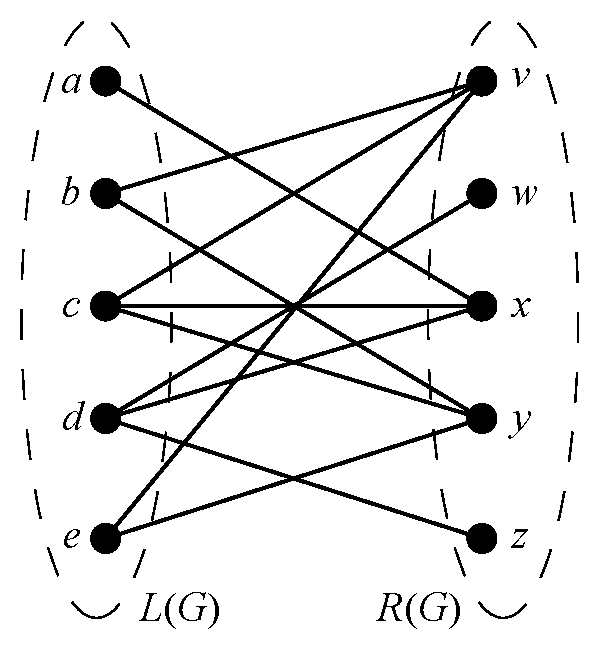
\includegraphics[width=2.5in]{MQ_bipartite_with_bottleneck}
\caption{$G$.\label{fig:bipartite_with_bneck}}
\end{figure}

\begin{solution}
It is not possible because $\set{a,b,c,e}$ is a bottleneck:
$\card{G(\set{a,b,c,e})} = \card{\set{v,x,y}} = 3 < 4 =
\card{\set{a,b,c,e}}$.  (It is easy to see that there are no
bottlenecks with exacty 1, 2, 3, or 5 vertices from $\leftbi{G}$.)

Another way to identify a bottlenexk is to observe that the
$\leftbi{G}$ and and $\rightbi{G}$ are the same size, and so there is
a bottleneck on the right iff there is one on the left.  So an
alternative answer is to observe that $\set{w,z}$ is a bottleneck in
the other direction: $\card{G^{-1}(\set{w,z})} =
\card{\set{d}} = 1 < 2 = \card{\set{w,z}}$.

\end{solution}

\examspace

\problempart The bipartite graph $H$ in
Figure~\ref{fig:deg_constrained_bipartite} has an easily verified
property that implies it has a matching that covers $\leftbi{H}$.
What is the property?

\begin{figure}[h]
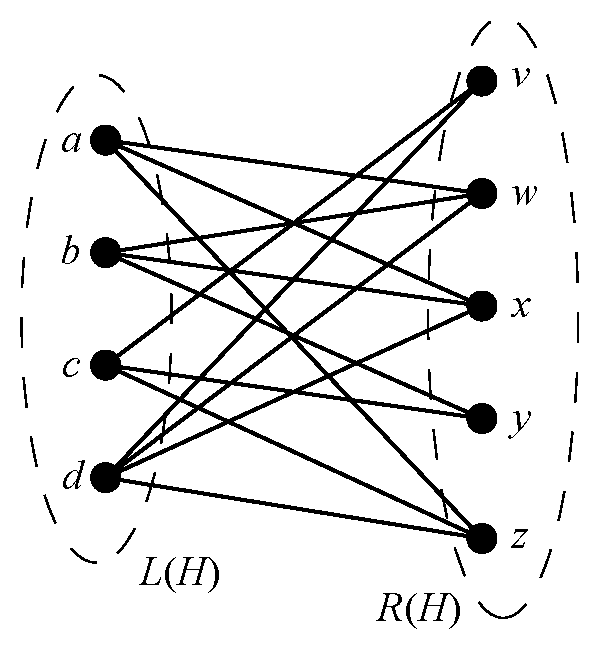
\includegraphics[width=2.5in]{MQ_degree_constrained_bipartite}
\caption{$H$.\label{fig:deg_constrained_bipartite}}
\end{figure}

\examspace[1in]
\begin{solution}
The graph is degree-constrained, and so
Theorem~\bref{lem:no_bottleneck_degree_constrained} ensure thata
matching exists.  In particular, Each vertex in $\leftbi{H}$ has
degree at least 3, while each vertex in $\rightbi{H}$ has degree at
most 3.

One matching, for example is:
\[
\edge{a}{z}, \edge{b}{w}, \edge{c}{v}, \edge{d}{x}.
\]

\end{solution}

\end{problemparts}
\end{problem}

\endinput
